\documentclass[11pt]{article}
\usepackage[a4paper,margin=1in]{geometry}
\usepackage[T1]{fontenc}
\usepackage[utf8]{inputenc}
% mathpazo dropped: Palatino math fonts not installed
\usepackage{microtype}
\usepackage{amsmath}
\usepackage{booktabs}
\usepackage{graphicx}
\usepackage{xcolor}
\usepackage{caption}
\usepackage{threeparttable}
\usepackage{placeins}
\usepackage{longtable,array,enumitem}
\usepackage[authoryear,round,sort]{natbib}
\definecolor{linkblue}{HTML}{1A0DAB}
\usepackage[colorlinks=true,citecolor=linkblue,linkcolor=linkblue,urlcolor=linkblue,breaklinks]{hyperref}
\usepackage{url}
\captionsetup{font=small,labelfont=bf,skip=4pt}
\graphicspath{{figures/}}
\newcommand{\code}[1]{\texttt{#1}}
\newcommand{\todo}[1]{\textcolor{red}{[TODO: #1]}}
% Table bodies are generated by tables.py. LaTeX's \input adds end-of-file hook tokens that
% break a tabular row, so the rows are read with the primitive instead.
\makeatletter\let\rawinput\@@input\makeatother
\newcommand{\pp}{\,pp}
\newcommand{\tool}{\tau}
\newcommand{\toolset}{\mathcal{T}}
\setlength{\tabcolsep}{4.5pt}
\newcommand{\aubfclargs}{1954}
\newcommand{\aubfcldesconly}{772}
\newcommand{\aubfcldesconlypct}{39.5}
\newcommand{\aubfclcopiedpct}{53}
\newcommand{\aubfcldesconlyparams}{41}
\newcommand{\aubfclsharedpct}{30}
\newcommand{\aubfcldescverbatim}{495}
\newcommand{\autsargs}{176}
\newcommand{\autsdesconly}{14}
\newcommand{\autsdesconlypct}{8.0}
\newcommand{\autscopiedpct}{61}
\newcommand{\autsdesconlyparams}{2}
\newcommand{\autssharedpct}{55}
\newcommand{\autsdescverbatim}{14}
\newcommand{\autauargs}{360}
\newcommand{\autaudesconly}{81}
\newcommand{\autaudesconlypct}{22.5}
\newcommand{\autaucopiedpct}{60}
\newcommand{\autaudesconlyparams}{6}
\newcommand{\autausharedpct}{47}
\newcommand{\autaudescverbatim}{95}%
\newcommand{\deight}{23.5, 25.5, 17.0, 17.0}
\newcommand{\deightrange}{17.0 to 25.5}
\newcommand{\deightvsdtworange}{9.0 to 22.0}
\newcommand{\deightvsdfourrange}{26.0 to 57.5}
\newcommand{\deightvsdzero}{-32.5, -25.0, -37.5, -55.0}
\newcommand{\deightvsdtwo}{-9.0, -11.0, -11.5, -22.0}
\newcommand{\deightvsdfour}{-35.0, -36.0, -26.0, -57.5}
\newcommand{\deightvsdtwobound}{14.0 to 28.5}
\newcommand{\deightvsdtwopmax}{0.0005}
\newcommand{\deightsixmax}{3.3}
\newcommand{\deightotherdrop}{10.1 to 37.6}
\newcommand{\dtwootherabs}{4.6}
\newcommand{\deightargacc}{62.2 to 79.3}
\newcommand{\dtwoargacc}{79.7 to 86.3}
\newcommand{\dzeroargacc}{90.7 to 94.4}
\newcommand{\lunadtworerun}{30.0}
\newcommand{\lunadtwodiff}{-2.5}
\newcommand{\lunadtwodiffci}{[-5.0, 0.0]}
\newcommand{\lunadtwodiscordant}{6 and 1}
\newcommand{\deightvslunarerun}{-6.5}
\newcommand{\deightvslunarerunci}{[-12.0, -1.5]}
\newcommand{\deightvslunarerunp}{0.0192}%
\newcommand{\tautrials}{4}
\newcommand{\tautrialdiff}{-3.5, +5.0, +1.5, -4.5}
\newcommand{\tautrialbound}{8.0 to 10.5}
\newcommand{\tautrialpmin}{0.10}
\newcommand{\tautrialdiffrange}{$-4.5$ to $+5.0$}
\newcommand{\taunoise}{0.0 to 14.0}%
\newcommand{\tautwodtwobounds}{12, 20, 16 and 22}
\newcommand{\tautwodtworange}{$+0.0$ to $+8.0$}
\newcommand{\tautwosinglebounds}{10 to 22}
\newcommand{\tautwootherrange}{$-6.0$ to $+8.0$}%
\newcommand{\sixsharemin}{63}
\newcommand{\sixsharemax}{91}%

% First-page header: the affiliation logo (figures/lucio-logo.png, from lucioai.com) over a rule.
\usepackage{fancyhdr}
\setlength{\headheight}{26pt}
\fancypagestyle{firstpage}{\fancyhf{}\lhead{
\includegraphics[height=20pt]{lucio-logo}}\cfoot{\thepage}\renewcommand{\headrulewidth}{0.4pt}}
% article's title block opens with a 2em gap; pull the title up to the header rule instead.
\makeatletter
\renewcommand{\@maketitle}{\newpage\null%
  \begin{center}\vspace*{-4em}\let\footnote\thanks  % glue after \null at the page top is discarded; this is not
  {\LARGE \@title \par}\vskip 1.2em%
  {\large \lineskip .5em \begin{tabular}[t]{c}\@author\end{tabular}\par}\vskip 0.6em%
  {\large \@date}\end{center}\par\vskip 1em}
\makeatother
\title{Which Parts of a Tool's Documentation Does a Model Actually Need?}
\hypersetup{pdftitle={Which Parts of a Tool's Documentation Does a Model Actually Need?}}
\author{\textbf{Randeep Singh}\\ Lucio AI\\ \texttt{randeep@lucioai.com}}

\date{\vspace{-3ex}}  % article still reserves a line for an empty date
\begin{document}
\maketitle
\thispagestyle{firstpage}
\suppressfloats[t]

\begin{abstract}
Function-calling interfaces document each tool with four pieces of text: a name, a description, parameter names and parameter descriptions. We ask what information in that text a model needs in multi-turn tasks and where it must be stated. On the Berkeley Function Calling Leaderboard (BFCL) we remove each component, then all four, for four models, with paired tests against a noise floor. Removing parameter descriptions is the only single removal that lowers task success for every model. Removing tool names or descriptions stays within noise, and removing all four leaves almost nothing. The damage is at argument construction, not selection, and comes from a few parameters whose descriptions alone stated an allowed value, a format or an entity type. Writing those constraints into the schema as \code{enum}, \code{pattern} and better parameter names restores baseline success with every description blank. On ToolSandbox and $\tau^2$-bench's airline domain, where an audit finds nearly every such constraint stated structurally or the value copied from the conversation, removing them has no detectable cost. Models need each constraint stated once, somewhere they can see it. On BFCL, the parameter descriptions happened to be the only place it was stated.
\end{abstract}

\section{Introduction}

Function calling is the standard way to connect a language model to software: the model is shown a list of tools, each a JSON Schema~\citep{jsonschema2020} with a name, a description and, per parameter, a name, a type and a description, and answers a user by emitting calls against that list~\citep{openai2023functioncalling,anthropic2024mcp}. Practitioners rewrite tool descriptions and a line of work studies how to write them well~\citep{hsieh2023tooldoc,yuan2025easytool,qu2025draft,guo2026rewrite}, but there is no controlled evidence about which parts of that text a model relies on inside a realistic multi-turn task with state to track and a few dozen tools to choose from.

We use the multi-turn base section of BFCL~\citep{patil2025bfcl,mao2024bfclv3}, keeping the tasks and execution environment fixed. We then vary the tool documentation presented to the model. Four models from four providers ran every task under every condition, three of them with reasoning on and off. All comparisons are paired at the task level and we repeat the baseline to measure run-to-run noise.

We then repeat the experiment on two other benchmarks: Apple's ToolSandbox~\citep{lu2024toolsandbox}, which documents every tool redundantly, and the airline domain of $\tau^2$-bench~\citep{barres2025tau2bench}, whose constraints are structural, to test the BFCL result where the same information is stated elsewhere.

Section~\ref{sec:background} fixes the vocabulary. A tool call involves two decisions, \emph{selecting} a tool and \emph{constructing} its arguments, and each needs different kinds of information: what a tool does, which values its parameters accept, and what values to supply. This information can appear in different places, which we call \emph{carriers}: the four text components, the structural fields of the schema, and the conversation. The experiment removes these carriers one at a time, and then all at once, to see how the information they carry affects tool use. We find:

\begin{itemize}\setlength\itemsep{0pt}
  \item \textbf{Removing parameter descriptions is the only single removal that hurts every model, because on BFCL they are the only statement of the constraints that matter} (Sections~\ref{sec:bfcl} and~\ref{sec:which}). Task success falls by 14 to 33.5 percentage points, significant for all seven configurations. The loss comes from six parameters whose description was the only statement of an allowed value, a format or an entity type. On the 91 tasks that use one of them, success falls by 31 to 74 points; on the other 109 tasks it barely moves, staying within run-to-run noise for six of the seven configurations.
  \item \textbf{The damage is at argument construction} (Section~\ref{sec:selection}). Models still pick the right tool as often as before. What falls, by 11 to 16 points, is the share of first calls that pick the right tool \emph{and} fill in the right arguments.
  \item \textbf{Structure carries the constraints as well as the prose did} (Section~\ref{sec:followup}). When the same constraints are written into the schema as \code{enum}s, \code{pattern}s and two more informative parameter names, every model returns to its baseline success with every description still blank.
  \item \textbf{Where no needed constraint is stated only in a description, removing descriptions has no detectable cost} (Sections~\ref{sec:audit} and~\ref{sec:nulls}). An audit of every ground-truth argument shows that on ToolSandbox and $\tau^2$-bench the constraints are carried by \code{enum}s or the values are copied from the conversation. On those two benchmarks, removing the descriptions changes no model's success by a detectable amount.
  \item \textbf{Tool-purpose information survives losing any one carrier, but not all of them} (Section~\ref{sec:d5}). Removing tool names, tool descriptions and parameter names together collapses tool selection on all three benchmarks. On $\tau^2$ airline the models then cancel the reservations they meant to look up, because the cancel and look-up tools have the same signature and nothing else is left to tell them apart.
  \item \textbf{Carriers are not always interchangeable, and reasoning does not compensate} (Sections~\ref{sec:bfcl} and~\ref{sec:behaviour}). Qwen3 loses 11.5 points when parameter names become generic even though every description stays in place, and the D2 drop is as large with reasoning on as with it off.
\end{itemize}

\section{Related work}\label{sec:related}

Tool use has progressed from inserted API calls~\citep{schick2023toolformer} and ReAct prompting~\citep{yao2023react} to models trained on tens of thousands of APIs~\citep{qin2024toolllm,patil2023gorilla}; \citet{qu2025survey} decompose tool use into planning, selection, calling and response generation, the framing behind Section~\ref{sec:bg-decisions}. API-Bank~\citep{li2023apibank} and BFCL's single-turn categories~\citep{yan2024bfcl} score individual calls; BFCL~V3~\citep{mao2024bfclv3}, $\tau$-bench~\citep{yao2025taubench} and ToolSandbox~\citep{lu2024toolsandbox} score a trajectory by its outcome.

Prior work treats documentation as one object to improve, by showing it can replace demonstrations~\citep{hsieh2023tooldoc} or by rewriting it~\citep{yuan2025easytool,qu2025draft,guo2026rewrite}; we ask which information in it is used and where it has to be. \citet{clouatre2026mcp} found, for two models, no measurable loss from moving parameter detail out of the tool description into per-parameter fields, the redundancy our D1 result shows. Robustness studies perturb the query, the toolkit, the interface or the outputs and find consistent degradation~\citep{rabinovich2025robustness,zheng2026toolrobustbench,xu2026agentperturb}, and \citet{chattopadhyay2026drift} find description and schema edits less harmful than distractor tools with overlapping descriptions, matching our D1/D3 nulls; none removes a component outright while holding the benchmark fixed. On the form of the interface, \citet{sigdel2026schemafirst} find that schema conditions reduce interface misuse but not semantic misuse, the design closest to our D6, and \citet{johnson2025nlt} find that replacing JSON tool calls with natural-language tool selection raises accuracy.

\section{Background}\label{sec:background}

\subsection{The function-calling interface}\label{sec:bg-interface}

Provider-native function calling~\citep{openai2023functioncalling} and the Model Context Protocol~\citep{anthropic2024mcp} share one format: each tool is a JSON object with a \code{name}, a \code{description} and a \code{parameters} JSON Schema~\citep{jsonschema2020}, and every model here receives exactly that serialised schema. Formally, a tool is a tuple $\tool = (n, d, P)$ of a name, a description and a parameter specification. Each $p \in P$ has a name, a type, a description and \emph{structural fields}, the ones JSON Schema defines with a fixed meaning: \code{required}, \code{default}, an \code{enum} of admissible values, a \code{pattern} a string must match, and nested specifications for object-typed parameters. The model is shown a tool set $\toolset = \{\tool_1, \ldots, \tool_K\}$ and answers with text or with calls $(n, a)$, where $a$ should conform to $P$.

The structural fields are machine-readable and have one meaning. The other four pieces of text, which we call the \emph{prose carriers} (names included, since each is free text with no fixed meaning), are the tool name, the tool description, the parameter names and the parameter descriptions. A description may say anything, including what a structural field could have said: ``Type of order (Buy/Sell)'' states an admissible-value set and ``Tags should start with \#'' a format. We call a constraint on an argument value \emph{structural} if a structural field expresses it and \emph{prose-only} if only a description states it. More generally, a \emph{carrier} is any place a piece of information is stated: the four prose carriers, the structural fields, and the conversation, that is, the user's request and the outputs of earlier calls.

\subsection{The interaction loop and its evaluation}\label{sec:bg-loop}

A tool-calling conversation alternates between a user and the model. Within a user \emph{turn} the model takes one or more \emph{steps}: it is sent the conversation so far and the tool set, and replies with calls or with text. Each call is executed against a backend, whose result or error is appended before the next step, and a text reply ends the turn. A \emph{stateful} backend lets a call change what later calls and turns see. Stateful benchmarks compare outcomes rather than calls. BFCL's multi-turn categories~\citep{mao2024bfclv3} replay a ground-truth call sequence on a copy of the backends and pass a turn only if the final states agree and any required outputs appear; $\tau$-bench~\citep{yao2025taubench} and ToolSandbox~\citep{lu2024toolsandbox} simulate the user with a language model and score the final state or the similarity to milestones. Outcome scoring is what makes a documentation ablation clean: the model may reach the required state by any sequence of calls, while the backend, the user and the ground truth are identical in every condition.

\subsection{Two decisions and what they need}\label{sec:bg-decisions}

At every step the model that acts makes two decisions: it \emph{selects} a tool $n \in \toolset$ and \emph{constructs} an argument object $a$ for it. The information this takes is of three kinds. \emph{Tool purpose}, what each tool does, is what selection needs. \emph{Argument constraints}, which values a parameter admits, in what format, and what kind of entity it names, are what construction needs beyond the parameter's type. \emph{Argument values} are the values themselves, which come from the user's request, from earlier results or from convention; they are not documentation, and a value copied from the conversation needs no constraint to be stated.

Each piece of information may be stated in several carriers at once. A tool's purpose, for example, is usually stated by its name, description and parameter list; an admissible set may be stated by an \code{enum} and again by a description. Where two carriers state the same thing, removing one leaves the other, and nothing should change. Where one carrier is the only statement, removing it removes the information: the model must then infer it, discover it by interacting with the backend (\emph{interactive recovery}), or fail. This is the prediction the experiment tests. Removing a carrier should cost nothing if what it carried is stated elsewhere or is not needed, and should cost at the decision that needs the content if it was the sole statement. In the trajectories, a \emph{selection failure} shows as the right tool never being called, a \emph{construction failure} as the right tool being called with wrong values, and recovery as a later call that corrects an earlier one.

\section{Experimental setup}\label{sec:setup}

\subsection{Benchmarks}

\paragraph{BFCL multi-turn base.} The \code{multi\_turn\_base} category~\citep{mao2024bfclv3} has 200 tasks of one to seven user turns (median four) over eight stateful Python backends. A task involves one or two backends and the model is shown every function of those backends, 18 to 39 tools (median 28). A turn passes if the backend state matches the state the ground-truth calls produce and any required outputs were produced, a task only if every turn passes, and a turn may take at most 20 steps. We used BFCL at commit \code{6ea57973}~\citep{gorilla-repo} at its default temperature of 0.001, unmodified.

\paragraph{ToolSandbox.} ToolSandbox~\citep{lu2024toolsandbox} (commit \code{c8571d7}) simulates the user with GPT-4o-2024-05-13, as in the original paper. Its tools are Python functions over a phone-like world whose schemas are generated from docstrings, so every description is one short line, and the score is a similarity in $[0,1]$ to the scenario's milestones. We run the 91 base scenarios that need no paid web API, each with 24 to 28 tools (Appendix~\ref{app:toolsandbox}).

\paragraph{$\tau^2$-bench airline.} The airline domain of $\tau^2$-bench~\citep{barres2025tau2bench} (version 2.0, commit \code{19f13ea}), the successor of $\tau$-bench~\citep{yao2025taubench}, has 50 tasks in which an agent shown 14 tools and the airline policy serves a user simulated by GPT-4.1, the benchmark's default. A task is rewarded 1 only if the final database state matches the state the ground-truth actions produce and, for the six tasks that require it, the agent's replies pass the benchmark's judge. Three of its parameters carry \code{enum}s and the values it needs are identifiers, codes and dates that the user states or a look-up returns, so its constraints are stated outside the prose (Appendix~\ref{app:tau2}).

\subsection{Documentation conditions}

\begin{table}[t]
\centering\small
\caption{Documentation conditions. Generic tool names are \code{tool\_01}\ldots\code{tool\_NN} in listing order; generic parameter names are \code{arg\_1}\ldots\code{arg\_n} per tool, recursively. Structural fields are kept throughout. $^{\dagger}$D1 also blanks the response-schema descriptions. $^{\ddagger}$D6 renames \code{cityA}/\code{cityB} to \code{zipcodeA}/\code{zipcodeB}.}
\label{tab:conditions}
\footnotesize\setlength{\tabcolsep}{4pt}
\begin{tabular}{lllll}
\toprule
 & Tool names & Tool descriptions & Parameter names & Parameter descriptions \\
\midrule
D0 & original & original & original & original \\
D1 & original & \textbf{removed}$^{\dagger}$ & original & original \\
D2 & original & original & original & \textbf{removed} \\
D3 & \textbf{generic} & original & original & original \\
D4 & original & original & \textbf{generic} & original \\
D5 & \textbf{generic} & \textbf{removed} & \textbf{generic} & \textbf{removed} \\
\addlinespace
D6 & original & original & original$^{\ddagger}$ & \textbf{removed}; constraints in schema \\
D7 & original & original & original & \textbf{removed}; six kept (Table~\ref{tab:wrongparams}) \\
D8 & original & original & \textbf{generic} & \textbf{removed} \\
\bottomrule
\end{tabular}
\end{table}

Each condition is an operation on the tuple $(n, d, P)$ that leaves the structural fields untouched (Table~\ref{tab:conditions}). D1 to D4 each remove one prose carrier, so each measures what that carrier stated that no other carrier did. D5 removes all four. It removes most of the semantics but not all of it: types, requiredness, enums, outputs and the user's request remain, and tools stay distinguishable by argument structure wherever that structure differs. When names are generic, the model's calls are translated back to the original names before the benchmark executes and scores them, so the backend and the evaluator see exactly what they would in D0. This holds on all three benchmarks. D6 and D7 blank every parameter description, as D2 does, in order to test the explanation that Section~\ref{sec:which} arrives at. D6 then writes every prose-only constraint of the BFCL schemas into a structural field: each parameter whose description holds an allowed-value list receives an \code{enum}, \code{post\_tweet.tags} and \code{mentions} receive the item patterns \code{\^{}\#} and \code{\^{}@}, and \code{estimate\_distance.cityA} and \code{cityB} are renamed \code{zipcodeA} and \code{zipcodeB}. D7 instead keeps only the six descriptions of Table~\ref{tab:wrongparams} and blanks the rest. D8 removes parameter names and parameter descriptions together while keeping tool names and descriptions. If the names stated nothing that the descriptions did not, D8 should perform like D2.

\subsection{Models and harness}

We evaluated GPT-6 Luna~\citep{openai2026gpt6}, Claude Haiku~5.5~\citep{anthropic2026haiku}, Qwen3-30B-A3B-Instruct-2507~\citep{yang2025qwen3} and Gemma~4 26B-A4B~\citep{google2026gemma4} through OpenRouter~\citep{openrouter}, all in native function-calling mode. On BFCL, Luna and Haiku reason by default and were also run with reasoning off; Gemma~4 does not reason by default and was also run with reasoning on; Qwen3 has no reasoning switch. That gives seven configurations. Each ran all 200 tasks under D0 to D5, and each model's default setting also ran D6 to D8. ToolSandbox and $\tau^2$ were run under D0 to D5 in each model's default setting. Each configuration's D0 to D5 were launched in one batch, so every ablation-versus-D0 comparison shares a batch. D6 and D7 ran three hours after their D0, a second Claude Haiku~5.5 run at D0 eight hours after the first (the run-to-run noise floor), and ToolSandbox and $\tau^2$ on the following two days. Two days after D0 came D8, a second Luna D2 run on BFCL and three further $\tau^2$ trials of D0 and D2. The harness subclasses each benchmark's OpenAI-compatible agent and differs from a stock run only in routing to OpenRouter, applying the condition, translating generic names back, and recording every trajectory in full (11\,200 BFCL trajectories, 2\,184 ToolSandbox plays and 2\,400 $\tau^2$ simulations). Four Qwen3 BFCL trajectories ended in a provider error and count as failures.

\subsection{Metrics and statistics}\label{sec:metrics}

Task success is each benchmark's own verdict. The behavioural metrics are statistics of the loop of Section~\ref{sec:bg-loop}, computed from the trajectories without any model-based judging. A \emph{call} is a tool call the benchmark decoded, and a \emph{step} is one model request. A call is \emph{on-path} if its tool appears in the ground truth, \emph{off-path} if not, and \emph{failed} if the backend returned an error. For each ground-truth call in turn $t$, a \emph{tool hit} means the model called that tool in any step of turns $0$ to $t$, and an \emph{exact hit} means one of those calls also had identical arguments (with no case folding, so \code{\"buy\"} does not match \code{\"Buy\"}). \emph{Tool-selection accuracy} is tool hits over ground-truth calls, and \emph{argument accuracy given the right tool} is exact hits over tool hits. For each failed task, the \emph{first divergence} is the earliest ground-truth call without an exact hit. It counts as a construction failure if the tool was called with other arguments and as a selection failure if the tool was never called. On $\tau^2$ the ground truth is the task's action list; on ToolSandbox it is the earliest milestone below similarity 1 that needs a tool. \emph{Recovery rate} is the share of tasks with at least one failed call that still passed.

\paragraph{Information audit.} For every argument of every ground-truth call, we record where the constraint on its value is stated. A parameter description \emph{states a constraint} if it gives an admissible-value list, a format, unit or range, or an entity type the parameter name does not give (zip codes for \code{cityA}); a single example (``such as 'ZFA04Y'\,'') or a restatement of the name is not a constraint. The judgement is per parameter and listed in Appendix~\ref{app:audit}. A structural field states a constraint if the parameter has an \code{enum} or \code{pattern} or is a boolean. A value is \emph{copied} if it occurs verbatim in the user's messages up to that turn or in the output of an earlier call, with outputs taken from a trajectory that passed the task at D0. ToolSandbox's relative-date reminders (``tomorrow 5PM'') are the one exception: the benchmark computes their expected timestamp from the clock at evaluation time, so the audit checks the timestamp the model passed in that trajectory. This gives five classes: description only; description and structure; structure only; none, copied; none, constructed. Separately, a tool's purpose counts as stated by its name, by its description, and by its signature when no tool offered alongside it has the same parameter names and types.

Every task appears in every condition, so each ablation is compared with D0 by an exact two-sided McNemar test~\citep{mcnemar1947} on the discordant cells, with a 95\% interval for the paired difference from a task-level bootstrap of 2\,000 resamples~\citep{efron1979}. With 35 BFCL comparisons (five ablations $\times$ seven configurations) the Bonferroni threshold is $p<0.0014$~\citep{dunn1961}. The 20 $\tau^2$ comparisons give $p<0.0025$. A null result is reported with its \emph{equivalence bound}, the largest change in either direction the interval allows.

\section{Results}\label{sec:results}

\subsection{BFCL: constraint information with a single carrier}\label{sec:bfcl}

\begin{table}[t]
\centering\small
\caption{BFCL task success (\%) per condition, 200 tasks per cell, with the paired change versus D0 in percentage points. Bold, starred cells are significant at the Bonferroni threshold $p<0.0014$ (exact McNemar test; discordant cells, intervals and $p$-values in Table~\ref{tab:paired}).}
\label{tab:success}
\setlength{\tabcolsep}{3pt}\scriptsize
\begin{tabular}{lrrrrrr}
\toprule
Model & D0 & D1 & D2 & D3 & D4 & D5 \\
\midrule
\rawinput tables/success.tex
\bottomrule
\end{tabular}
\end{table}

\paragraph{Removing parameter descriptions is the only single removal that hurts every model.} Every configuration in Table~\ref{tab:success} has the same shape: a small dip at D1, a large drop at D2, no change at D3 and a collapse at D5. D2 and D5 are significant for all seven configurations at the corrected threshold. The D2 discordant cells are lopsided: in each configuration, between 42 and 75 tasks pass in D0 but fail in D2, while only 5 to 16 pass in D2 but fail in D0 (Table~\ref{tab:paired}). D1 and D3 have discordant cells of similar size in both directions and every interval includes zero, although all seven D1 differences are negative ($-2.5$ to $-6.0$\pp). D4 is harmless for Luna and Gemma~4. It costs Qwen3 11.5\pp\ ($p=0.001$), even though every description Qwen3 could read stayed in place, and it shows an apparent $+11.0$\pp\ gain for Haiku with reasoning that is absent with reasoning off.

\paragraph{Two identical runs differ by about as much as D1 or D3.}\label{sec:noise}
\newcommand{\rerunsecond}{56.5}
\newcommand{\rerunboth}{92}
\newcommand{\rerunaonly}{9}
\newcommand{\rerunbonly}{21}
\newcommand{\rerundiff}{+6.0}
\newcommand{\rerunp}{0.0428}%%
Claude Haiku~5.5's second D0 run passed \rerunsecond\% of tasks against 50.5\% in the first: \rerunaonly\ tasks passed only in the first run and \rerunbonly\ only in the second ($\Delta=\rerundiff$\pp, $p=\rerunp$; Table~\ref{tab:rerun}). This gap is the floor against which single-condition differences must be read. D3 sits at it, and so does D4 for three of the four models; both are null results. D1 is a possible small cost. Haiku's D1 gap widens to $-8.5$\pp\ ($p=0.008$) when measured against the second run, and D1 is negative for all seven configurations, but one run per condition cannot resolve a difference of a few points. D2 and D5 are an order of magnitude above the floor and significant against either run. Reasoning shifts baseline success but leaves the D2 drop in place. The three pairs that differ only in the reasoning switch show D2 drops of $-23.5$ and $-22.0$\pp\ (Luna with reasoning on and off), $-14.0$ and $-19.5$\pp\ (Haiku) and $-33.0$ and $-33.5$\pp\ (Gemma~4), even though reasoning budgets respond to the interface (Table~\ref{tab:tokens}).

\subsection{Where the information is stated: an audit of the ground truth}\label{sec:audit}

\begin{table}[t]
\centering\footnotesize
\caption{Information audit. For every argument of every ground-truth call: where the constraint on its value is stated (the five classes of Section~\ref{sec:metrics}), how many of the arguments with a description constraint nonetheless have their value verbatim in the conversation, the kinds of constraint the descriptions state, and the number of parameters whose description is the only statement of a constraint (listed in Appendix~\ref{app:audit}).}
\label{tab:audit}
\setlength{\tabcolsep}{2.8pt}\scriptsize
\resizebox{\textwidth}{!}{%
\begin{tabular}{l rrr rrrrr r rrr r}
\toprule
 & & & & \multicolumn{5}{c}{constraint stated in} & \multicolumn{4}{c}{description constraints} & \\
\cmidrule(lr){5-9}\cmidrule(lr){10-13}
Benchmark & calls & args & params & desc.\ only & desc.\,+\,struct. & struct.\ only & none, copied & none, constructed & verbatim & enum & format & entity & desc.-only params \\
\midrule
\rawinput tables/audit.tex
\bottomrule
\end{tabular}}
\end{table}

\paragraph{On BFCL two fifths of the ground-truth arguments have a constraint stated only in a description; on the other two benchmarks the constraints are structural or the values are copied.} Table~\ref{tab:audit} classifies the \aubfclargs\ arguments of BFCL's 1\,142 ground-truth calls, the \autsargs\ values that ToolSandbox's milestones pin, and the \autauargs\ arguments of $\tau^2$'s 142 ground-truth actions. On BFCL, \aubfcldesconly\ arguments (\aubfcldesconlypct\%), spread over \aubfcldesconlyparams\ parameters, have a constraint whose only statement is the description. These are 217 allowed-value lists written as prose, 496 formats, units, ranges or ``no path'' rules, and 59 entity types that the parameter name hides. The six parameters of Section~\ref{sec:which} are among the \aubfcldesconlyparams. Half of all BFCL arguments (\aubfclcopiedpct\%) are copied from the conversation and need no constraint at all; so are \aubfcldescverbatim\ of the \aubfcldesconly\ description-constrained ones. The remaining 277 arguments, led by \code{ignitionMode}, \code{order\_type} and the date and pedal-position formats, are the cases where a description is the only route to the value. ToolSandbox has \autsdesconly\ description-only arguments (\autsdesconlypct\%), all of them the POSIX-timestamp format of \code{reminder\_timestamp}, whose value a conversion tool returns. A further 32 of its values are booleans, and \autscopiedpct\% are copied. $\tau^2$ has \autaudesconly\ description-only arguments (\autaudesconlypct\%), airport-code and date formats, but \autaudescverbatim\ of its 101 description-constrained values appear verbatim in the user's messages or in an earlier look-up. Its cabin and flight-type lists are stated both in the description and in an \code{enum}, and \autaucopiedpct\% of its values are copied. Tool purpose is stated by name and description for every tool on every benchmark, and additionally by a signature no other tool shares for 70\% of BFCL's ground-truth tool instances, 45\% of ToolSandbox's and 53\% of $\tau^2$'s (Table~\ref{tab:purpose}).

\subsection{ToolSandbox and $\tau^2$-bench: no detectable cost where the information is stated elsewhere}\label{sec:nulls}

\paragraph{Removing parameter descriptions has no detectable cost on either benchmark, for a different reason on each.} On ToolSandbox, D2 changes mean similarity by $-6.3$ to $+2.0$ points depending on the model (sign-flip $p\geq 0.07$) and leaves the share of exactly solved scenarios unchanged for every model (Appendix~\ref{app:toolsandbox}). The audit says why. Of its 176 pinned values, the 14 whose only constraint is a description are timestamps that an earlier conversion call returns. In the passing D0 trajectories all \autsdescverbatim\ are that call's output, so the format is enforced by the tool that produces the value and the model only has to copy it. The information D2 removes was not needed. On $\tau^2$, D2 changes success by \tautwodtworange\pp\ ($p\geq 0.34$; Table~\ref{tab:tau2}). With 50 tasks per condition, the single-trial intervals bound the change at \tautwodtwobounds\pp\ for Luna, Haiku, Qwen3 and Gemma~4. Running D0 and D2 for four trials per model narrows this: the trial-averaged change is \tautrialdiffrange\pp\ and the bounds tighten to \tautrialbound\pp\ (Appendix~\ref{app:tau2}), which is below the smallest D2 effect seen on BFCL. Here the information was needed but was stated elsewhere. Cabin and flight type keep their \code{enum}s, and 95 of the 101 description-constrained values, airport codes and dates, appear verbatim in the user's messages or in the reservation the agent has just looked up. The two benchmarks therefore speak to different things. ToolSandbox's descriptions hold no argument constraint, so its D2 null says only that tool-purpose information is stated redundantly; $\tau^2$ shows one constraint surviving in an \code{enum} when its prose statement goes. D1, D3 and D4 are likewise nulls on both benchmarks. On $\tau^2$ every change is within \tautwootherrange\pp\ with bounds of \tautwosinglebounds\pp\ (Table~\ref{tab:tau2paired}), and on ToolSandbox within a few points, except for Gemma~4's $-6.0$ at D3 ($p=0.003$). Qwen3's BFCL D4 cost does not reappear on $\tau^2$ ($-4.0$\pp, bound 16).

\subsection{Removing every carrier of a tool's purpose collapses selection on all three benchmarks}\label{sec:d5}

D5 is significant for every BFCL configuration ($-47.0$ to $-73.5$\pp), for every ToolSandbox model ($-39$ to $-49$ similarity points, $p<0.0001$) and for three of the four models on $\tau^2$ ($-30$ to $-68$\pp; Gemma~4's $-14.0$ has $p=0.12$). The failures are failures of selection. On BFCL, tool-selection accuracy falls to 16 to 60\%, and most failed tasks begin with a ground-truth tool that is never called (Table~\ref{tab:divergence}), whereas at D2 most begin with the right tool called with wrong arguments. On ToolSandbox, among the 75 to 78 plays per model below similarity 1, the earliest unmet milestone needs a tool that was never called in 63 to 70 of them, against 5 to 9 at D0 (Table~\ref{tab:toolsandboxdivergence}). On $\tau^2$, 15 to 39 of the 36 to 50 failed tasks per model begin with an action's tool never called, and nearly all of them contain a state-changing call that the ground truth does not (Table~\ref{tab:tau2divergence}). The mechanism is visible in the calls. \code{cancel\_reservation} and \code{get\_reservation\_details} both take a single \code{reservation\_id}, so once names and descriptions are gone nothing in the schema tells them apart, and every model's look-ups turn into cancellations (Appendix~\ref{app:tau2}). Tool-purpose information is stated redundantly enough to survive any one removal; D5 removes every statement of it at once.

\section{Analysis}\label{sec:analysis}

Section~\ref{sec:bg-decisions} says where parameter descriptions could matter: at selection, at construction, or in interactive recovery. The BFCL trajectories tell the three apart.

\subsection{Selection versus construction}\label{sec:selection}

\paragraph{D2 leaves selection intact and damages construction.} Between D0 and D2, tool-selection accuracy moves by only 2.6 to 8.8 points, and part of that is cascade: a turn derailed by a wrong argument may never reach its later tools. Argument accuracy given the right tool, by contrast, falls for every configuration, from 90.7--94.7\% to 79.5--86.3\% (Figure~\ref{fig:selection}a,b). The first call of each task is free of cascade (Figure~\ref{fig:selection}c). In D2 the right tool is chosen first at least as often as in D0 for every configuration, but the share of first calls with the right tool and the right arguments falls by 11.0 to 16.0 points. The first divergence of failed tasks tells the same story (Figure~\ref{fig:divergence}): relative to D0, construction failures rise by 34 to 66 per configuration and selection failures by only 2 to 11. D5, by contrast, fails at selection (Section~\ref{sec:d5}).

\subsection{Which descriptions matter}\label{sec:which}

\paragraph{Six parameters carry the effect, and each description was the only statement of a constraint.} Table~\ref{tab:wrongparams} links each new argument error under D2 to the description that was removed. The same six parameters lead for every configuration, and each of their descriptions held a prose-only constraint in the sense of Section~\ref{sec:bg-interface}: an allowed-value list (``Buy/Sell'' for \code{order\_type}, ``START, STOP'' for \code{ignitionMode}), an entity type the name hides (\code{cityA} and \code{cityB} take zip codes, not city names), or a format (\code{tags} start with \code{\#}, \code{mentions} with \code{@}). Without the description, models wrote \code{\"buy\"} for \code{\"Buy\"}, passed city names where zip codes were expected, or folded the hashtag into the tweet body. At task level the effect sits on the tasks that use these parameters. The ground truth of 91 of the 200 tasks uses at least one of the six, and \sixsharemin\ to \sixsharemax\% of the tasks that pass in D0 and fail in D2 are among those 91. On the 91 tasks the D2 drop is 30.8 to 73.6\pp. On the other 109 tasks it is between $-10.1$ and $+4.6$\pp, within the noise floor for six of the seven configurations (Table~\ref{tab:sixparam}). Parameter descriptions matter here less as explanations of meaning than as the place where this benchmark happens to keep its enums, formats and entity conventions. Section~\ref{sec:followup} tests whether a structural field can hold them instead.

\subsection{Restoring the structure without the prose}\label{sec:followup}

\paragraph{Writing the constraints into the schema restores baseline with every description blank.} If the descriptions that matter are the sole statements of constraints the schema could express, two things should follow: D6 should perform like D0, and D7 should recover most but not all of the loss. Both hold (Figure~\ref{fig:followup}, Table~\ref{tab:followup}). D6 lands within 3.5 points of D0 for every model; no D6--D0 difference is significant, and every D6--D2 difference is, recovering 17.5 to 31.0 points. D7 recovers most of the D2 loss but stays 4 to 10 points below D0 for three models. What still goes wrong under D7 is the remaining prose-only enums that only D6 converts, led by \code{lockDoors.door}. D6 is one move, from a parameter description to a structural field. It shows that structure carried these constraints as well as prose did, and nothing more, because other placements were not tested. The models read the constraint rather than having it enforced on them. Counting every value emitted for the 13 constrained parameters, the share outside the constraint is 37 to 69\% in D2 and at most 0.7\% in D6 for every model. Three models were already at 0.0\% in D0, where the constraint was prose that no decoder could enforce. Enforcement is therefore not needed to explain the recovery, which matters because enforcement is not free~\citep{constrainttax2026}.

\paragraph{Removing parameter names and descriptions together costs more than either.} D8 blanks every description and makes every parameter name generic, keeping tool names and descriptions. Success falls to \deightrange\%, which is \deightvsdtworange\pp\ below D2 (every $p\leq\deightvsdtwopmax$; Table~\ref{tab:names}) and \deightvsdfourrange\pp\ below D4. The extra loss is not the six parameters' doing. On the 109 tasks that use none of them, where D2 moved success by at most \dtwootherabs\pp, D8 costs \deightotherdrop\pp\ (Table~\ref{tab:sixparam}). The parameters that newly go wrong, \code{book\_flight}'s arguments and \code{lockDoors.unlock}, are ones whose values the model can no longer assign to the right slot once both the name and the description are gone. What a parameter \emph{is} was stated twice, by its name and by its description. Removing either alone cost nothing (D4, for three models) or cost only the constraints that the descriptions alone stated (D2). Removing both leaves the type as the only statement. D8 ran two days after D2. As a check on that gap, a second Luna D2 run launched on the same day as D8 differs from the first D2 run by \lunadtwodiff\pp, and D8 is \deightvslunarerun\pp\ below it ($p=\deightvslunarerunp$).

\subsection{Behaviour, recovery and failure outcomes}\label{sec:behaviour}

The third possibility of Section~\ref{sec:bg-decisions} is that a model compensates for missing information by interacting with the backend. Under the single ablations it does not. D2 adds 0.1 to 2.8 calls per task over D0, and what changes is the composition of the calls rather than their number: failed calls per task rise from at most 0.03 to between 0.10 and 0.51 (Appendix~\ref{app:behaviour}). Recovery after an execution error is poor in D2, at 5 to 22\% of the 19 to 30 tasks that contained one, and all but absent in D5, where six configurations recovered none of their 17 to 102 such tasks. Under D5 two opposite behaviours appear. Haiku and Luna with reasoning end the first turn without any call in 22 to 35\% of tasks, while Qwen3, and Gemma~4 with reasoning, keep probing until the step cap. Neither behaviour passes tasks (case studies in Appendix~\ref{app:cases}).

\section{Discussion}\label{sec:discussion}

\paragraph{For tool designers.} The descriptions whose removal hurt were not explaining what a parameter means. They were the only statement of an allowed-value list, a format rule or an entity convention that JSON Schema could have expressed as an \code{enum}, a \code{pattern} or a better name. This suggests the audit of Section~\ref{sec:audit} as a design check. For every parameter description, ask whether it states a constraint that the structural fields do not; if it does, state the constraint there as well, and keep the prose for what structure cannot say. Qwen3's D4 result is the caution. The information was still in the descriptions, yet replacing the names with \code{arg\_N} cost 11.5\pp, so carriers are not interchangeable for every model.

\paragraph{Why tool names and descriptions could be removed one at a time.} A tool's purpose is stated by its name, by its description and, for most tools, by a signature no other tool shares. Removing any one of these leaves the others. D5 shows the information was used, since removing all of them collapses selection on every benchmark. The design cannot rank names, descriptions and parameter names against each other, because each is one redundant carrier of the same information. It does show where the redundancy ends. $\tau^2$'s cancel and look-up tools, and ToolSandbox's four \code{set\_*\_status} tools, share a signature, and once names and descriptions are gone the models act on the wrong one. On $\tau^2$ the wrong one was destructive: models cancelled reservations they meant to look up rather than ask. That is a safety observation as much as a selection failure, and a case for studying how agents should act when a tool's effect is uncertain. With semantically overlapping tools~\citep{chattopadhyay2026drift,rabinovich2025robustness}, single removals should start to matter. Interaction does not substitute for the missing information. Declining to act fails because the evaluator requires the state change, probing fails at the step cap, and recovery is poor even in D2. Whether dry runs, more steps or structured diagnostics~\citep{sigdel2026schemafirst} would help is open.

\paragraph{For benchmark designers.} The D2 effect flows through a dozen parameters in three backends and disappears when their constraints are written into the schema. A benchmark that encoded its enums and formats structurally, as $\tau^2$ does, would isolate task understanding from prose parsing. Conversely, BFCL's multi-turn checker compares backend attributes with Python equality while its single-turn checker normalises case (Appendix~\ref{app:tables}), so \code{"buy"} for \code{"Buy"} fails a task.

\section{Limitations}\label{sec:limitations}

\paragraph{One run per condition.} Two identical runs disagree on tens of tasks (Section~\ref{sec:noise}), so this design cannot resolve differences of a few points. The D2, D5 and D6-versus-D2 effects are an order of magnitude larger than that. The repeated D0 run exists only for Claude Haiku~5.5 on BFCL. D8 was launched two days after the D2 and D4 runs it is compared with, and the same-day Luna D2 rerun (Section~\ref{sec:followup}) is the only check on that gap. ToolSandbox was run once, and $\tau^2$ once for D1, D3, D4 and D5, each with a simulated user whose variation enters every difference. $\tau^2$'s 50 tasks bound a single-trial null at \tautwosinglebounds\pp\ and the four-trial D2 null at \tautrialbound\pp, which is coarser than the BFCL noise floor.

\paragraph{The placement claim rests on one move.} D6 moves constraints from a parameter description into \code{enum}, \code{pattern} and a parameter name. No other placement was tested: a constraint stated in the tool description, in the system prompt or in a tool's output might or might not serve as well, so ``any carrier'' is not supported. The redundancy between parameter names and parameter descriptions was tested directly only by D8, run once per model in its default setting.

\paragraph{D5 keeps the structure; the metrics are strict; the audit is a judgement.} D5's collapse is partly a property of evaluators that cap steps and score final state. The audit was written after all three benchmarks had been run and their results seen, so it classifies after the fact and predicted nothing. Its ``states a constraint'' is a per-parameter reading of the schema text, written out so it can be disputed, and ``copied'' is verbatim occurrence, which misses a value the user stated in another form.

\paragraph{Provider and reasoning settings were not fully controlled.} Routing was left to OpenRouter, a third of Qwen3's BFCL trajectories touched a second provider (the D2 effect is present on both subsets), and the reasoning switch sets no effort level.

\section{Conclusion}\label{sec:conclusion}

Most tool documentation is redundant. What a tool does is stated in its name, in its description and usually in its signature. On three benchmarks that information survived the loss of any one of these, with two model-specific exceptions (Sections~\ref{sec:bfcl} and~\ref{sec:nulls}), but never the loss of all of them. Constraints on argument values are different. On BFCL, an allowed-value list, a format or an entity type was often stated in one parameter description and nowhere else, and removing that description removed the information, for the same six parameters in every model. Writing the same constraints into the schema restored baseline success with every description blank. On two benchmarks whose constraints were already structural, or whose values the conversation supplied, the same removal had no detectable cost. It is the information, not the prose, that the models need. Tool designers should state each constraint in a structural field as well as in words, and benchmark designers should know that a score can rest on where a convention happens to be written.

\section*{Reproducibility statement}
\begin{sloppypar}
The harness, the condition definitions (including the exact D6 transformation), the audit and analysis code and the paper sources are at \url{https://github.com/Eazydraft/exp-tool-semantics-ablation}, with BFCL, ToolSandbox and $\tau^2$-bench as pinned submodules. Every number, table and figure is computed from the 15\,784 trajectory files under \path{runs/main/trajectories/}, each holding the exact tool schemas sent, every raw request and response, the benchmark's state and the verdict; \texttt{./run.sh browse} shows any trajectory with the schemas as the model saw them.
\end{sloppypar}

\section*{Acknowledgements}
This study used the BFCL harness, backends and evaluator~\citep{patil2025bfcl,gorilla-repo}, ToolSandbox~\citep{lu2024toolsandbox} and $\tau^2$-bench unchanged; we thank their authors. Models were accessed through OpenRouter~\citep{openrouter}.

\bibliographystyle{plainnat}
\bibliography{references}

\clearpage
\appendix
\begin{center}{\LARGE\bfseries APPENDIX}\end{center}
\vspace{0.5em}

\section{Additional results on BFCL}\label{app:tables}

\begin{figure}[h]
\centering
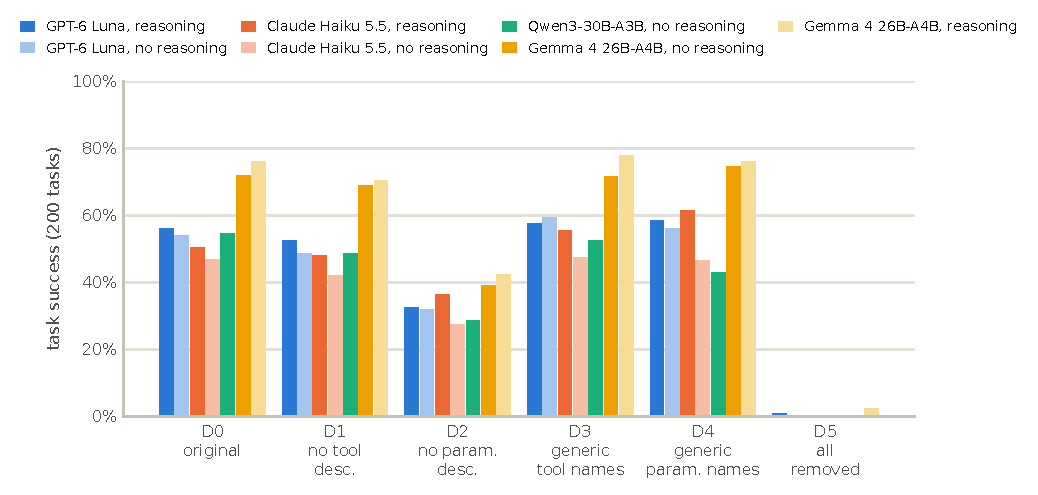
\includegraphics[width=\linewidth]{fig1_success}
\caption{Task success rate by condition for the seven configurations (lighter tint: the non-default reasoning setting). Each bar is 200 tasks; bars within a configuration are paired.}
\label{fig:success}
\end{figure}

\begin{figure}[h]
\centering
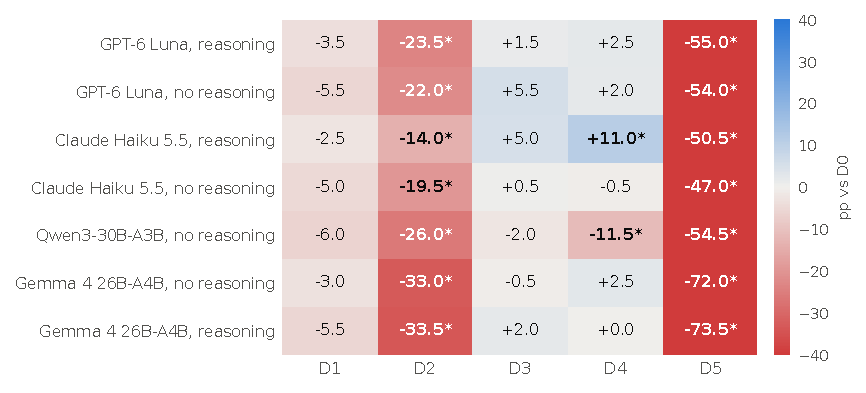
\includegraphics[width=0.62\linewidth]{fig2_heatmap}
\caption{Change in task success relative to D0, in percentage points. Starred, bold cells are significant at $p<0.0014$ (exact McNemar test, Table~\ref{tab:paired}).}
\label{fig:heatmap}
\end{figure}

\begin{table}[h]
\centering\footnotesize
\caption{Each ablation versus D0 on the same 200 tasks: the two discordant cells, the paired difference $\Delta$ in percentage points with its 95\% task-level bootstrap interval (2\,000 resamples), the exact two-sided McNemar $p$, and the Bonferroni verdict for 35 comparisons ($p<0.0014$). Each configuration's D1 to D5 share a launch batch with its D0.}
\label{tab:paired}
\setlength{\tabcolsep}{3pt}\scriptsize
\resizebox{\textwidth}{!}{%
\begin{tabular}{llrrrrrrrl}
\toprule
Model & Cond. & both pass & D0 only & abl.\ only & both fail & $\Delta$\pp & 95\% CI & McNemar $p$ & $p<0.0014$ \\
\midrule
\rawinput tables/paired.tex
\bottomrule
\end{tabular}}
\end{table}

\begin{table}[h]
\centering\footnotesize
\caption{Run-to-run noise: a repeated D0 run of Claude Haiku~5.5 against the first, and each condition against both D0 runs. Same 200 tasks, same settings, eight hours apart; the second run is the only repeated D0 run in the study, and no comparison with it shares a batch.}
\label{tab:rerun}
\begin{tabular}{lrrrrrrr}
\toprule
Comparison & both pass & first only & second only & both fail & $\Delta$\pp & 95\% CI & McNemar $p$ \\
\midrule
\rawinput tables/rerun.tex
\bottomrule
\end{tabular}
\end{table}

\begin{table}[h]
\centering\small
\caption{Reasoning tokens per task by condition, mean over the 200 tasks.}
\label{tab:tokens}
\begin{tabular}{lrrrrrr}
\toprule
Model & D0 & D1 & D2 & D3 & D4 & D5 \\
\midrule
\rawinput tables/tokens.tex
\bottomrule
\end{tabular}
\end{table}

\begin{table}[h]
\centering\small
\caption{Documentation sensitivity score $S_m=\frac{1}{N}\sum_i (P_{m,0}-P_{m,i})/P_{m,0}$, the mean relative drop from D0 over D1--D4 and over D1--D5. Because it averages a large D2 loss with near-zero changes elsewhere, it understates the D2 effect and is reported for completeness only.}
\label{tab:robustness}
\begin{tabular}{lrr}
\toprule
Model & $S$ (D1--D4) & $S$ (D1--D5) \\
\midrule
\rawinput tables/robustness.tex
\bottomrule
\end{tabular}
\end{table}

\paragraph{Memorisation check.}
Across the 1\,515 to 3\,927 tool calls each default configuration made in D3 and D5, and the 3\,886 to 7\,055 calls each reasoning variant made in D3, D4 and D5, no configuration emitted a single original tool name, and across D4 and D5 none emitted a single original parameter name. The only non-generic strings were eight malformed generic names from Qwen3 (\code{tool\_6} for \code{tool\_06}) and ten non-generic argument keys from Luna with reasoning.

\begin{sloppypar}
\paragraph{Checker strictness.} At the pinned commit, \code{standardize\_string} in \path{bfcl_eval/eval_checker/ast_eval/ast_checker.py} removes spaces and punctuation and lower-cases both sides before the single-turn comparison, whereas \code{\_compare\_instances} in \path{bfcl_eval/eval_checker/multi_turn_eval/multi_turn_checker.py} tests every public attribute of the model's backend instance against the ground-truth instance with Python equality, and the multi-turn response checker matches serialised outputs without normalisation.
\end{sloppypar}

\paragraph{Haiku's D4 gain.} Haiku with reasoning passes 29 tasks only in D4 against 7 only in D0 ($p=0.0003$). The gain is absent with reasoning off ($-0.5$\pp), shrinks to $+5.0$\pp\ ($p=0.13$) against the repeated D0 run, and is diffuse: the 29 tasks span 16 backend combinations, 19 involve the six parameters of Table~\ref{tab:wrongparams} and 10 do not, and their D0 failures begin with a wrong argument in 12 cases, a never-called tool in 7 and no identifiable divergence in 10. We offer no mechanism for it.

\begin{figure}[h]
\centering
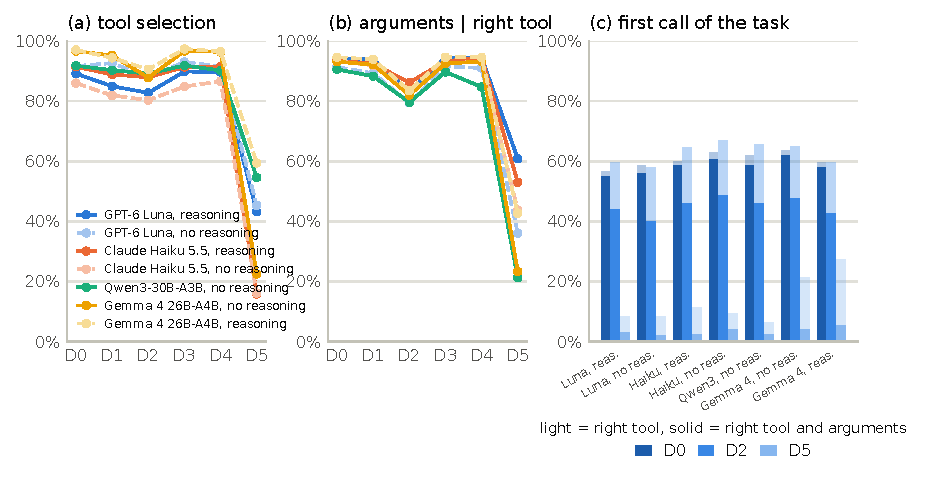
\includegraphics[width=0.8\linewidth]{fig3_selection_vs_args}
\caption{(a) Tool-selection accuracy. (b) Argument accuracy given the right tool. (c) First call of the task: share of tasks whose first call used a ground-truth tool (light) and used it with the ground-truth arguments (solid), for D0, D2 and D5. Numbers in Table~\ref{tab:selection}.}
\label{fig:selection}
\end{figure}

\begin{table}[h]
\centering\small
\caption{Tool selection versus argument construction (\%). ``Sel.'' is tool-selection accuracy, ``Arg.'' argument accuracy given the right tool, ``1st tool'' the share of tasks whose first call used a ground-truth tool, ``1st exact'' the share whose first call matched a ground-truth call exactly.}
\label{tab:selection}
\resizebox{\textwidth}{!}{%
\begin{tabular}{l rrrr rrrr rrrr}
\toprule
 & \multicolumn{4}{c}{D0} & \multicolumn{4}{c}{D2} & \multicolumn{4}{c}{D5} \\
\cmidrule(lr){2-5}\cmidrule(lr){6-9}\cmidrule(lr){10-13}
Model & Sel. & Arg. & 1st tool & 1st exact & Sel. & Arg. & 1st tool & 1st exact & Sel. & Arg. & 1st tool & 1st exact \\
\midrule
\rawinput tables/selection.tex
\bottomrule
\end{tabular}}
\end{table}

\begin{figure}[h]
\centering
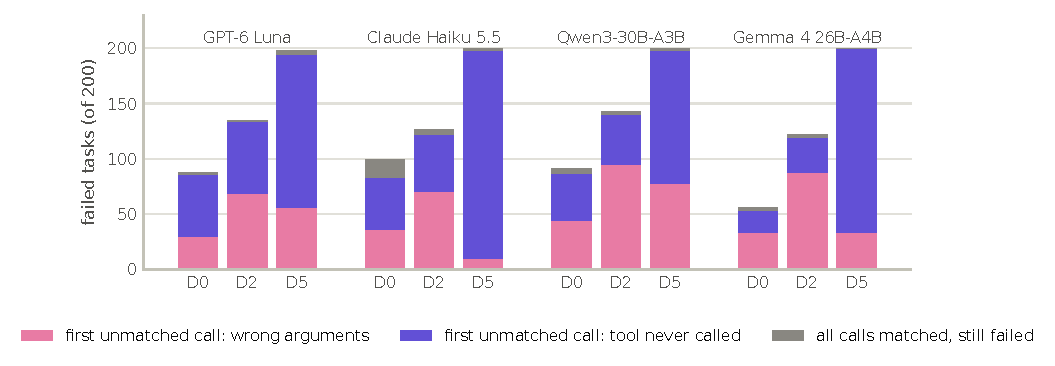
\includegraphics[width=\linewidth]{fig4_divergence}
\caption{Earliest divergence in failed tasks: the first ground-truth call without an exact match, classified by whether the tool was called with wrong arguments (construction failure) or never called (selection failure); ``all calls matched'' means every ground-truth call was matched but the task still failed, usually through extra state-changing calls or a call made in a later turn than required.}
\label{fig:divergence}
\end{figure}

\begin{table}[h]
\centering\small
\caption{Earliest divergence among failed BFCL tasks (counts). ``W.A.'': wrong arguments; ``N.C.'': tool never called; ``None'': every ground-truth call matched but the task failed.}
\label{tab:divergence}
\begin{tabular}{l rrr rrr rrr}
\toprule
 & \multicolumn{3}{c}{D0} & \multicolumn{3}{c}{D2} & \multicolumn{3}{c}{D5} \\
\cmidrule(lr){2-4}\cmidrule(lr){5-7}\cmidrule(lr){8-10}
Model & W.A. & N.C. & None & W.A. & N.C. & None & W.A. & N.C. & None \\
\midrule
\rawinput tables/divergence.tex
\bottomrule
\end{tabular}
\end{table}

\begin{table}[h]
\centering\footnotesize
\caption{Parameters whose values go wrong when their description is removed. For every ground-truth call matched by the right tool but wrong arguments, the differing parameters were recorded. Counts are pooled over the seven configurations (1\,400 task runs per condition), sorted by D2$-$D0; D2 counts per configuration on the right ($-$: reasoning off, $+$: on). The second column quotes the description D2 removed.}
\label{tab:wrongparams}
\begin{threeparttable}
\scriptsize\setlength{\tabcolsep}{2.6pt}
\resizebox{\textwidth}{!}{%
\begin{tabular}{p{4.1cm} p{5.2cm} rr rrrrrrr}
\toprule
Tool.parameter & Removed description & D2 & D0 & Luna & Luna$^{-}$ & Haiku & Haiku$^{-}$ & Qwen3 & Gemma & Gemma$^{+}$ \\
\midrule
\rawinput tables/wrongparams.tex
\bottomrule
\end{tabular}}
\end{threeparttable}
\end{table}

\begin{table}[h]
\centering\footnotesize
\caption{Success (\%) on the 91 tasks whose ground truth uses at least one of the six parameters of Table~\ref{tab:wrongparams} (``six'') and on the other 109 (``other''). The first column counts the tasks that pass in D0 and fail in D2 and, of those, how many are six-parameter tasks. D6 to D8 exist for each model's default reasoning setting.}
\label{tab:sixparam}
\resizebox{\textwidth}{!}{%
\begin{tabular}{l r rr rr rr rr rr}
\toprule
 & D0-only tasks & \multicolumn{2}{c}{D0} & \multicolumn{2}{c}{D2} & \multicolumn{2}{c}{D6} & \multicolumn{2}{c}{D7} & \multicolumn{2}{c}{D8} \\
\cmidrule(lr){3-4}\cmidrule(lr){5-6}\cmidrule(lr){7-8}\cmidrule(lr){9-10}\cmidrule(lr){11-12}
Model & six / all & six & other & six & other & six & other & six & other & six & other \\
\midrule
\rawinput tables/sixparam.tex
\bottomrule
\end{tabular}}
\end{table}

\begin{figure}[h]
\centering
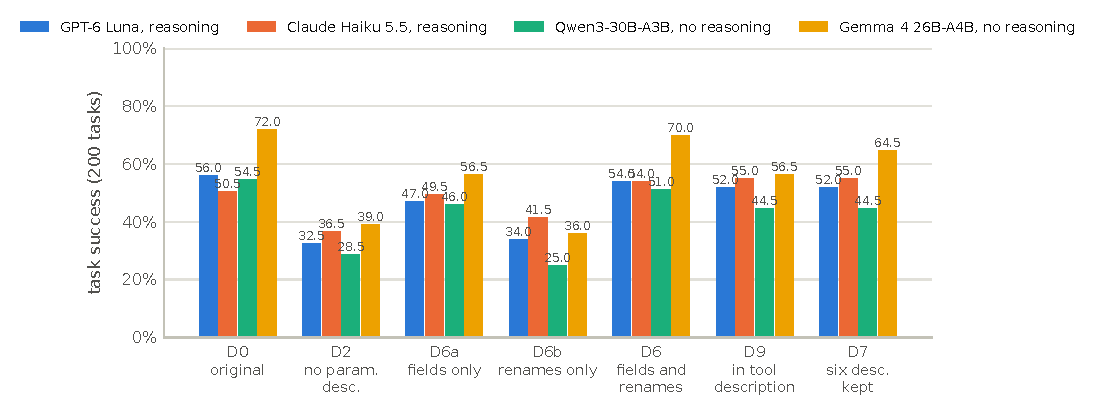
\includegraphics[width=0.8\linewidth]{fig10_followup}
\caption{D6 and D7, each model in its default reasoning setting. Both blank every parameter description, as D2 does. D6 moves the prose-only constraints into the schema; D7 keeps only the six descriptions of Table~\ref{tab:wrongparams}. Paired tests in Table~\ref{tab:followup}.}
\label{fig:followup}
\end{figure}

\begin{table}[h]
\centering\footnotesize
\caption{D6 and D7 against D0 and against D2 on the same 200 tasks (each model in its default reasoning setting): success of the base condition and of D6 or D7, the discordant cells, the paired difference with its 95\% bootstrap interval, and the exact McNemar $p$. D6 and D7 were launched three hours after D0 to D5 and do not share a batch with them.}
\label{tab:followup}
\setlength{\tabcolsep}{3.5pt}
\resizebox{\textwidth}{!}{%
\begin{tabular}{llrrrrrrr}
\toprule
Model & Comparison & base \% & D6/D7 \% & base only & D6/D7 only & $\Delta$\pp & 95\% CI & $p$ \\
\midrule
\rawinput tables/followup.tex
\bottomrule
\end{tabular}}
\end{table}

\begin{table}[h]
\centering\footnotesize
\caption{D8 (generic parameter names and blank parameter descriptions together, tool names and descriptions kept) against D0, D2 and D4 on the same 200 tasks (each model in its default reasoning setting): success of the base condition and of D8, the discordant cells, the paired difference with its 95\% bootstrap interval, its equivalence bound and the exact McNemar $p$. D8 was launched two days after D0 to D5 and shares a batch with none of them.}
\label{tab:names}
\setlength{\tabcolsep}{3.5pt}
\resizebox{\textwidth}{!}{%
\begin{tabular}{llrrrrrrrr}
\toprule
Model & Comparison & base \% & D8 \% & base only & D8 only & $\Delta$\pp & 95\% CI & bound & $p$ \\
\midrule
\rawinput tables/names.tex
\bottomrule
\end{tabular}}
\end{table}

\FloatBarrier
\section{The information audit in detail}\label{app:audit}

\begin{table}[h]
\centering\footnotesize
\caption{How many carriers state each tool's purpose. A tool instance is one tool in one task's ground truth; every tool has a name and a description, and its signature counts as a third carrier when no tool offered alongside it in that task has the same parameter names and types. The last column lists the tools that most often share a signature.}
\label{tab:purpose}
\setlength{\tabcolsep}{4pt}
\begin{tabular}{lrrrrp{6.2cm}}
\toprule
Benchmark & tool instances & 3 carriers & 2 carriers & shared & most often shared \\
\midrule
\rawinput tables/purpose.tex
\bottomrule
\end{tabular}
\end{table}

\paragraph{Parameters whose description is the only statement of a constraint.} The audit's per-parameter judgement is the table \code{CONSTRAINT\_KIND} in \path{ablation/audit.py}; the parameters it lists that occur in the ground truth are, per benchmark:
\begin{sloppypar}\begin{description}[leftmargin=1.2em,itemsep=1pt,font=\normalfont\itshape]\small
\rawinput tables/auditparams.tex
\end{description}\end{sloppypar}
On BFCL, a boolean is the only structural constraint any ground-truth parameter carries, so no argument has a constraint stated both in prose and in structure. ``Copied'' takes outputs from the first configuration whose D0 run passed the task; 71 BFCL ground-truth calls, 48 ToolSandbox pinned values and 26 $\tau^2$ actions could not be located in such a trajectory and use every output the trajectory received.

\FloatBarrier
\section{Tool-use behaviour on BFCL}\label{app:behaviour}

\begin{figure}[h]
\centering
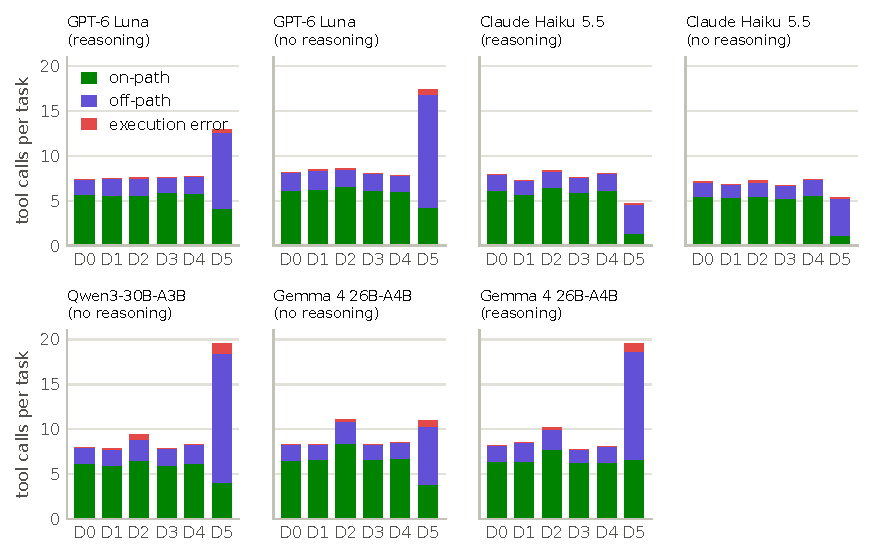
\includegraphics[width=\linewidth]{fig5_calls}
\caption{Composition of tool calls per task (mean over all 200 tasks, failures included): on-path calls, off-path calls that executed without error, and calls that returned an execution error.}
\label{fig:calls}
\end{figure}

\begin{figure}[h]
\centering
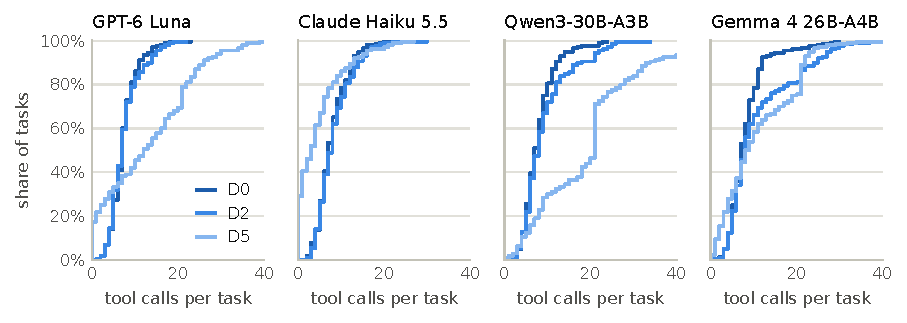
\includegraphics[width=\linewidth]{fig7_ecdf}
\caption{Empirical cumulative distribution of tool calls per task for D0, D2 and D5, all 200 tasks per curve. D2 shifts the distribution only slightly; D5 pulls it in opposite directions by model, Haiku rising steeply at 0 to 3 calls and Qwen3 stretching to the step cap.}
\label{fig:ecdf}
\end{figure}

\begin{figure}[h]
\centering
\begin{minipage}[t]{0.5\linewidth}\centering
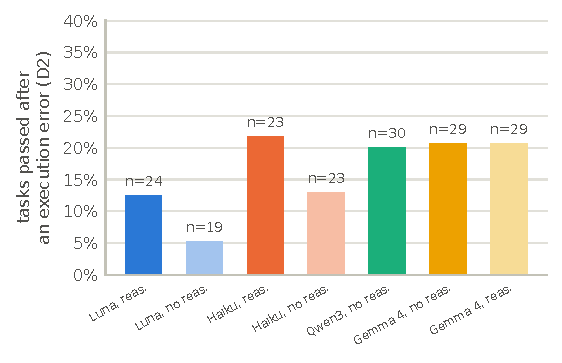
\includegraphics[width=\linewidth]{fig9_recovery}
\end{minipage}\hfill
\begin{minipage}[t]{0.47\linewidth}\centering
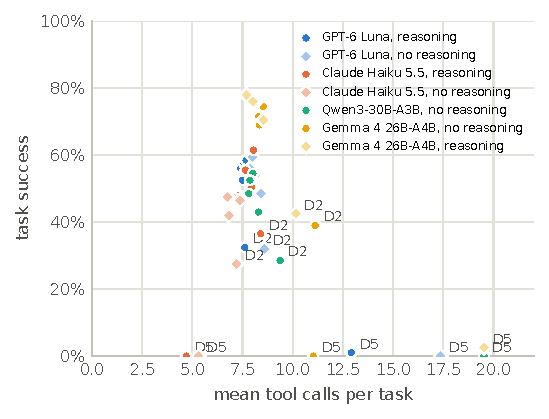
\includegraphics[width=\linewidth]{fig8_frontier}
\end{minipage}
\caption{\textbf{Left:} recovery after an execution error in D2: share of tasks containing at least one failed call that still passed, with the number of such tasks. D0 denominators are 1 to 4 tasks and not comparable. \textbf{Right:} task success against mean tool calls per task, one point per configuration and condition. D0 through D4 sit at 7 to 9 calls per task; D5 moves points right (Qwen3, Luna, Gemma~4) or left (Haiku) without moving them up.}
\label{fig:recovery}
\end{figure}

\begin{figure}[h]
\centering
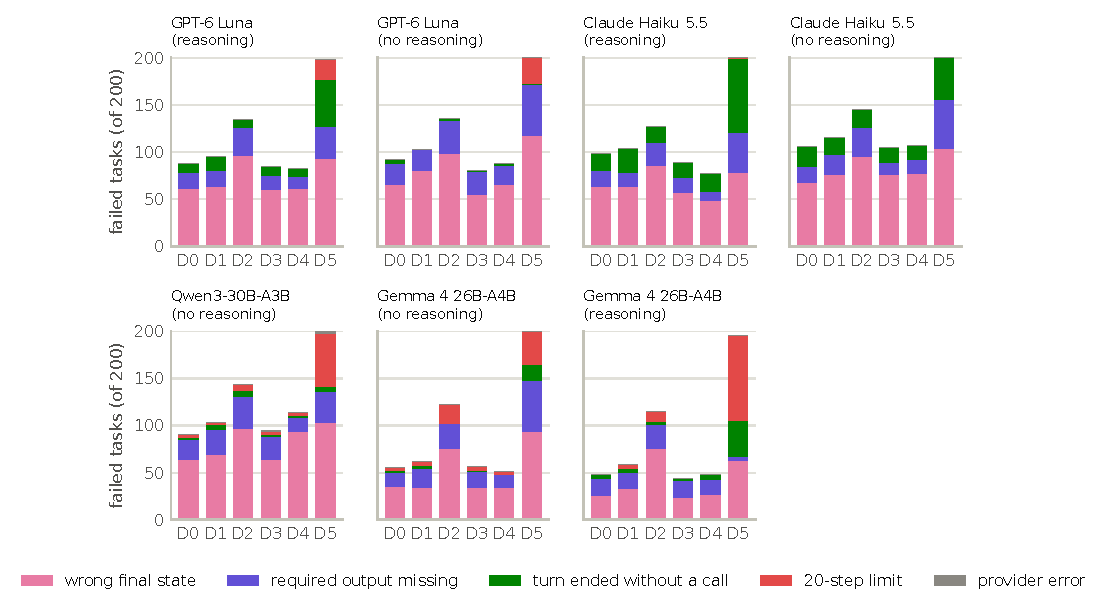
\includegraphics[width=\linewidth]{fig6_failures}
\caption{BFCL's terminal error per failed task, by condition. These are outcomes, not causes: a wrong final state can come from a wrong tool, a wrong argument or a missed step.}
\label{fig:failures}
\end{figure}

\begin{table}[h]
\centering\footnotesize
\caption{Tool-use behaviour, mean per task over all 200 tasks (failures included). A repeated call has identical tool and arguments to an earlier call in the same task; ``calls/pass'' is the mean over passing tasks only.}
\label{tab:behaviour}
\resizebox{\textwidth}{!}{%
\begin{tabular}{llrrrrrrrr}
\toprule
Model & Cond. & calls & steps & on-path & off-path & failed & repeated & distinct tools & calls/pass \\
\midrule
\rawinput tables/behaviour.tex
\bottomrule
\end{tabular}}
\end{table}

\begin{table}[h]
\centering\small
\caption{Recovery after an execution error: share of tasks containing at least one failed call that still passed, with the number of such tasks in parentheses.}
\label{tab:recovery}
\begin{tabular}{lrrrrrr}
\toprule
Model & D0 & D1 & D2 & D3 & D4 & D5 \\
\midrule
\rawinput tables/recovery.tex
\bottomrule
\end{tabular}
\end{table}

\begin{table}[h]
\centering\footnotesize
\caption{Terminal error assigned by BFCL per failed task. ``State'': wrong final state; ``Output'': required output missing; ``Empty'': turn ended without a tool call; ``Limit'': 20-step limit reached; ``Provider'': inference error.}
\label{tab:failures}
\begin{tabular}{llrrrrrr}
\toprule
Model & Cond. & State & Output & Empty & Limit & Provider & Total failed \\
\midrule
\rawinput tables/failures.tex
\bottomrule
\end{tabular}
\end{table}

\paragraph{D5 behaviour in detail.} Haiku makes fewer calls than in D0 (4.7 against 7.9 with reasoning, 5.3 against 7.1 without), makes no call in the first turn of 34.5\% of tasks (18.0\% without reasoning), and most of its calls are off-path. Qwen3 makes 19.5 calls per task over 15.6 distinct tools of the roughly 28 available, with an execution error in 51\% of tasks. Luna with reasoning sits between (12.9 calls, no first-turn call in 22\% of tasks), as does Gemma~4 without reasoning (11.0 calls); the other setting of each probes instead (Luna without reasoning 17.4 calls, Gemma~4 with reasoning 19.5). BFCL's terminal errors follow the strategy: Haiku's and Luna's D5 failures with reasoning are dominated by turns that ended without a tool call (78 and 50 tasks), Qwen3's by the 20-step limit (57) and Gemma~4's by a wrong final state after probing (94); without reasoning Luna probes to a wrong final state (118) and Haiku splits (104 wrong states, 44 silent turns), and Gemma~4 with reasoning hits the step limit in 90 tasks. In D2 the extra failures are almost all wrong final states (for example 35 $\to$ 76 for Gemma~4): the model acted, but on the wrong values.

\FloatBarrier
\section{ToolSandbox: setup and results}\label{app:toolsandbox}

\paragraph{Setup.} ToolSandbox's 1\,032 scenarios are 129 base scenarios in eight variants that vary distraction tools and apply the benchmark's own augmentations; we take the 91 base scenarios that need none of the five tools backed by a paid web API, in the variant that offers every tool the scenario does not withhold (24 to 28 tools per scenario; 28 in 73 of the 91), so that tool selection is part of every task as on BFCL. The user simulator is reached through OpenRouter with the same seed in every condition. ToolSandbox executes each call as a Python statement named after the provider's tool-call id; two providers return ids that are not valid identifiers, which the unmodified harness turns into a syntax error on every call, so the harness rewrites such ids before execution. When a model emits arguments that are not valid JSON, ToolSandbox aborts the scenario; like its own runner we score it 0 (27 of 2\,184 plays, all Qwen3's). We report the mean similarity and the share of scenarios at similarity 1.0, and test paired differences with a sign-flip permutation test on the similarity and McNemar's test on the binary outcome.

\begin{figure}[h]
\centering
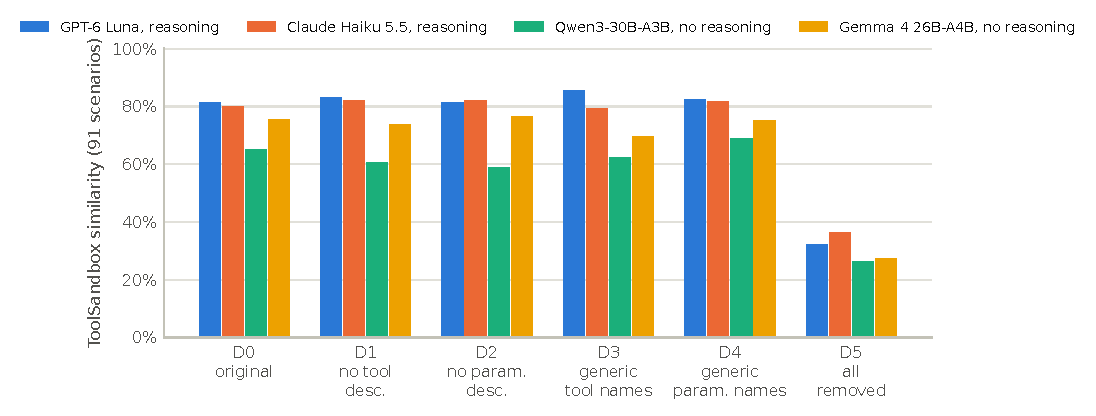
\includegraphics[width=\linewidth]{fig11_toolsandbox}
\caption{ToolSandbox mean similarity by condition (91 scenarios per bar). Removing any single component leaves every model within a few points of its baseline; removing all four costs 39 to 49 points.}
\label{fig:toolsandbox}
\end{figure}

\begin{table}[h]
\centering\footnotesize
\caption{ToolSandbox results. Left: mean similarity ($\times 100$) over the 91 scenarios; right: share solved exactly (similarity 1.0).}
\label{tab:toolsandbox}
\setlength{\tabcolsep}{3.6pt}
\begin{tabular}{lrrrrrrrrrrrr}
\toprule
 & \multicolumn{6}{c}{mean similarity} & \multicolumn{6}{c}{solved exactly (\%)} \\
\cmidrule(lr){2-7}\cmidrule(lr){8-13}
Model & D0 & D1 & D2 & D3 & D4 & D5 & D0 & D1 & D2 & D3 & D4 & D5 \\
\midrule
\rawinput tables/toolsandbox.tex
\bottomrule
\end{tabular}
\end{table}

\paragraph{Results.} Removing parameter descriptions (D2) changes mean similarity by $-0.3$, $+2.0$, $-6.3$ and $+0.9$ points for Luna, Haiku, Qwen3 and Gemma~4 (sign-flip $p\geq 0.07$; Table~\ref{tab:toolsandboxpaired}), and the share solved exactly is unchanged for every model (discordant cells 5/5, 2/1, 3/4, 2/2). D1 ($+1.4$, $+2.0$, $-4.2$, $-1.8$) and D4 are likewise within a few points, and so is D3 except for Gemma~4, which loses 6.0 points ($p=0.003$) and seven exactly-solved scenarios against none gained ($p=0.016$), the one single-component effect to reach nominal significance. D5 costs 39 to 49 points for every model ($p<0.0001$).

The single-component nulls are what the audit of Section~\ref{sec:audit} predicts. Across the 72 parameters of the 28 tools an agent can see, none carries an allowed-value list the schema lacks; the only prose constraints are formats (``POSIX timestamp'', ``in 24hr format''), and most restate the parameter name (\code{reminder\_timestamp\_lowerbound}, \code{hour}). Identifiers the tools exchange (\code{person\_id}) are returned by earlier calls, so the agent copies rather than constructs them. The one suggestive exception points the same way: Qwen3's $-6.3$ is concentrated in the 36 \emph{canonicalization} scenarios (70.0 to 58.5; Table~\ref{tab:toolsandboxcats}), where the user states a date, duration or unit in surface form that the agent must convert before calling, that is, where a format convention has to be applied.

Tool selection survives every single-component condition. Taking as reference each model's D0 scenarios with similarity at least 0.9 in which it called a tool (54, 49, 53 and 41 for Haiku, Gemma~4, Luna and Qwen3), the share in which the ablated run calls every tool the D0 run used is 0.87 to 0.91 for Haiku under D1 to D4, 0.76 to 0.90 for Gemma~4, 0.74 to 0.83 for Luna and 0.66 to 0.76 for Qwen3, against 0.00 to 0.13 under D5. What D5 removes is the ability to tell 24 to 28 tools apart by anything but argument structure, and much of that is shared: six tools take no arguments, eight take one, and the four \code{set\_*\_status} tools all take a single boolean. Table~\ref{tab:toolsandboxdivergence} gives the first-divergence split: at D0 to D4 most plays below similarity 1 have every tool milestone met and differ from the reference only in the wording of a reply, and the 9 to 23 plays with an unmet tool milestone split between the tool called with other arguments and the tool never called; at D5, 63 to 70 plays per model never call the tool the first unmet milestone needs. The collapse looks as it does on BFCL: scenarios in which the agent never calls a tool rise from 6, 3, 7 and 0 (Luna, Haiku, Qwen3, Gemma~4) to 27, 19, 16 and 34; scenarios that run to the 30-message cap rise from 2 to 23 for Luna and 10 to 32 for Qwen3; two models mostly fall silent (Haiku, Gemma~4) and two probe to the limit (Luna, Qwen3). Because the user is simulated, its token usage rises by 40 to 180\% in D5.

Two features of ToolSandbox limit what can be read from it. Its 18 \emph{insufficient-information} scenarios, where the correct behaviour is to ask rather than act, score low for every model in every condition (24 to 74 at D0) and move by less than a point under D2. And the user is an LLM with the same seed in every condition but not deterministic, so each paired difference includes user noise; the sign-flip tests account for it but are not a substitute for a repeated run, which we did not make.

\begin{table}[h]
\centering\footnotesize
\caption{ToolSandbox: every ablation against D0, paired over the 91 scenarios. Similarity columns are means ($\times 100$) with the bootstrap 95\% CI of the paired difference and a sign-flip permutation $p$ (10\,000 permutations); exact-match columns give the share at similarity 1.0, the discordant cells (only in D0 / only in the ablation) and the exact McNemar $p$.}
\label{tab:toolsandboxpaired}
\setlength{\tabcolsep}{2.6pt}
\begin{tabular}{llrrrcrrrrr}
\toprule
 & & \multicolumn{5}{c}{mean similarity} & \multicolumn{4}{c}{solved exactly} \\
\cmidrule(lr){3-7}\cmidrule(lr){8-11}
Model & Cond. & D0 & abl. & $\Delta$ & 95\% CI & $p$ & D0 \% & abl. \% & D0/abl. only & McNemar $p$ \\
\midrule
\rawinput tables/toolsandboxpaired.tex
\bottomrule
\end{tabular}
\end{table}

\begin{table}[h]
\centering\footnotesize
\caption{ToolSandbox mean similarity ($\times 100$) by scenario category, D0 against D2. Categories are ToolSandbox's own and overlap ($n$ is the number of the 91 scenarios in each).}
\label{tab:toolsandboxcats}
\setlength{\tabcolsep}{4pt}
\begin{tabular}{lrrrrrrrrr}
\toprule
 & & \multicolumn{2}{c}{GPT-6 Luna} & \multicolumn{2}{c}{Claude Haiku 5.5} & \multicolumn{2}{c}{Qwen3-30B-A3B} & \multicolumn{2}{c}{Gemma 4 26B-A4B} \\
\cmidrule(lr){3-4}\cmidrule(lr){5-6}\cmidrule(lr){7-8}\cmidrule(lr){9-10}
Category & $n$ & D0 & D2 & D0 & D2 & D0 & D2 & D0 & D2 \\
\midrule
\rawinput tables/toolsandboxcats.tex
\bottomrule
\end{tabular}
\end{table}

\begin{table}[h]
\centering\small
\caption{Earliest divergence among ToolSandbox plays below similarity 1 (counts). The earliest unmet milestone that needs a tool: that tool was called (``W.A.'') or never called (``N.C.''); ``tools ok'': every tool milestone met and only a reply milestone unmet; ``abort'': ToolSandbox aborted the play on malformed arguments.}
\label{tab:toolsandboxdivergence}
\footnotesize\setlength{\tabcolsep}{3pt}
\begin{tabular}{l rrrr rrrr rrrr}
\toprule
 & \multicolumn{4}{c}{D0} & \multicolumn{4}{c}{D2} & \multicolumn{4}{c}{D5} \\
\cmidrule(lr){2-5}\cmidrule(lr){6-9}\cmidrule(lr){10-13}
Model & W.A. & N.C. & tools ok & abort & W.A. & N.C. & tools ok & abort & W.A. & N.C. & tools ok & abort \\
\midrule
\rawinput tables/toolsandboxdivergence.tex
\bottomrule
\end{tabular}
\end{table}

\FloatBarrier
\section{$\tau^2$-bench airline: setup and results}\label{app:tau2}

\paragraph{Setup.} $\tau^2$-bench is used unmodified from its repository at version 2.0 (commit \code{19f13ea}), in text mode on the airline domain, with the benchmark's default step and error limits and one trial per task. The agent is the benchmark's own LLM agent with the tool schemas passed through the condition on the way out and the model's calls translated back on the way in, so the environment and the evaluator see original names. The user is simulated by GPT-4.1 and the communicate-information checks, which six of the 50 tasks carry, are judged by GPT-5.5 as the benchmark pins them; both are reached through OpenRouter like the agent, at temperature 0. The reward basis of the airline domain is the database state and the communicate checks, so the natural-language-assertion judge never runs. The four models ran in their default reasoning setting under D0 to D5 in one batch on 4 November 2026; no repeated run was made.

\begin{table}[h]
\centering\small
\caption{$\tau^2$-bench airline task success (\%) per condition, 50 tasks per cell, with the paired change versus D0. Bold, starred cells are significant at the Bonferroni threshold for the 20 $\tau^2$ comparisons, $p<0.0025$ (exact McNemar test; discordant cells, intervals, equivalence bounds and $p$-values in Table~\ref{tab:tau2paired}).}
\label{tab:tau2}
\setlength{\tabcolsep}{3pt}\scriptsize
\begin{tabular}{lrrrrrr}
\toprule
Model & D0 & D1 & D2 & D3 & D4 & D5 \\
\midrule
\rawinput tables/tau2.tex
\bottomrule
\end{tabular}
\end{table}

\begin{table}[h]
\centering\footnotesize
\caption{$\tau^2$-bench airline: each ablation versus D0 on the same 50 tasks: the discordant cells, the paired difference with its 95\% bootstrap interval, the equivalence bound (the largest change in either direction the interval allows), the exact McNemar $p$ and the Bonferroni verdict for 20 comparisons ($p<0.0025$).}
\label{tab:tau2paired}
\setlength{\tabcolsep}{3pt}\scriptsize
\resizebox{\textwidth}{!}{%
\begin{tabular}{llrrrrrrrrl}
\toprule
Model & Cond. & both pass & D0 only & abl.\ only & both fail & $\Delta$\pp & 95\% CI & $|\Delta|<$ & McNemar $p$ & $p<0.0025$ \\
\midrule
\rawinput tables/tau2paired.tex
\bottomrule
\end{tabular}}
\end{table}

\begin{table}[h]
\centering\footnotesize
\caption{$\tau^2$-bench airline: D0 and D2 run for several trials (trial 1 is the run of Table~\ref{tab:tau2}; the later trials were launched two days after it, each with its own seed). Success is averaged over trials; $\Delta$ is the mean over tasks of the per-task difference in trial-averaged success, with its bootstrap 95\% interval, equivalence bound and a sign-flip permutation $p$ (10\,000 permutations). The last column is the range over pairs of D0 trials of the absolute difference in success, the benchmark's own trial-to-trial variation.}
\label{tab:tau2trials}
\setlength{\tabcolsep}{4pt}
\begin{tabular}{lrrrrrrrr}
\toprule
Model & trials & D0 \% & D2 \% & $\Delta$\pp & 95\% CI & bound & $p$ & D0 trial pairs \\
\midrule
\rawinput tables/tau2trials.tex
\bottomrule
\end{tabular}
\end{table}

\begin{table}[h]
\centering\footnotesize
\caption{$\tau^2$-bench airline: where the reward is lost. Failed tasks, those failing the database check, those failing a communicate check, both; simulations ending at the step limit or the error limit; mean tool calls per task. Every other simulation ended with the agent or the user stopping.}
\label{tab:tau2breakdown}
\begin{tabular}{llrrrrrrr}
\toprule
Model & Cond. & failed & DB fail & comm.\ fail & both & step limit & error limit & calls/task \\
\midrule
\rawinput tables/tau2breakdown.tex
\bottomrule
\end{tabular}
\end{table}

\begin{table}[h]
\centering\small
\caption{Earliest divergence among failed $\tau^2$ tasks (counts). ``W.A.'': a ground-truth action's tool called with other arguments; ``N.C.'': never called; ``None'': every action matched but the task failed; ``write'': failed tasks containing a state-changing call (booking, cancellation, update or certificate) that the ground truth does not.}
\label{tab:tau2divergence}
\footnotesize\setlength{\tabcolsep}{3pt}
\begin{tabular}{l rrrr rrrr rrrr}
\toprule
 & \multicolumn{4}{c}{D0} & \multicolumn{4}{c}{D2} & \multicolumn{4}{c}{D5} \\
\cmidrule(lr){2-5}\cmidrule(lr){6-9}\cmidrule(lr){10-13}
Model & W.A. & N.C. & None & write & W.A. & N.C. & None & write & W.A. & N.C. & None & write \\
\midrule
\rawinput tables/tau2divergence.tex
\bottomrule
\end{tabular}
\end{table}

\paragraph{What D5 does on airline.} Every D5 simulation of Luna, Haiku and Qwen3 still ends by a normal agent or user stop with about five tool calls, so the models act rather than stall; Gemma~4 hits the error limit in 10 tasks and the step limit in one. The calls change tool: \code{cancel\_reservation}, which takes the reservation id alone, is called 126, 149, 101 and 54 times by Luna, Haiku, Qwen3 and Gemma~4 against 11, 7, 25 and 16 at D0, while \code{get\_reservation\_details}, which has the same single parameter, falls from 113, 136, 114 and 140 calls to 8, 10, 20 and 66. Gemma~4 is the partial exception because it probes instead, calling the zero-argument \code{list\_all\_airports} and \code{calculate} tools 112 and 72 times, which is also why its D5 drop is smaller and not significant. The communicate checks fail in one to six tasks per cell in every condition and do not carry the effect.

\FloatBarrier
\section{Case studies}\label{app:cases}

\begin{figure}[h]
\centering
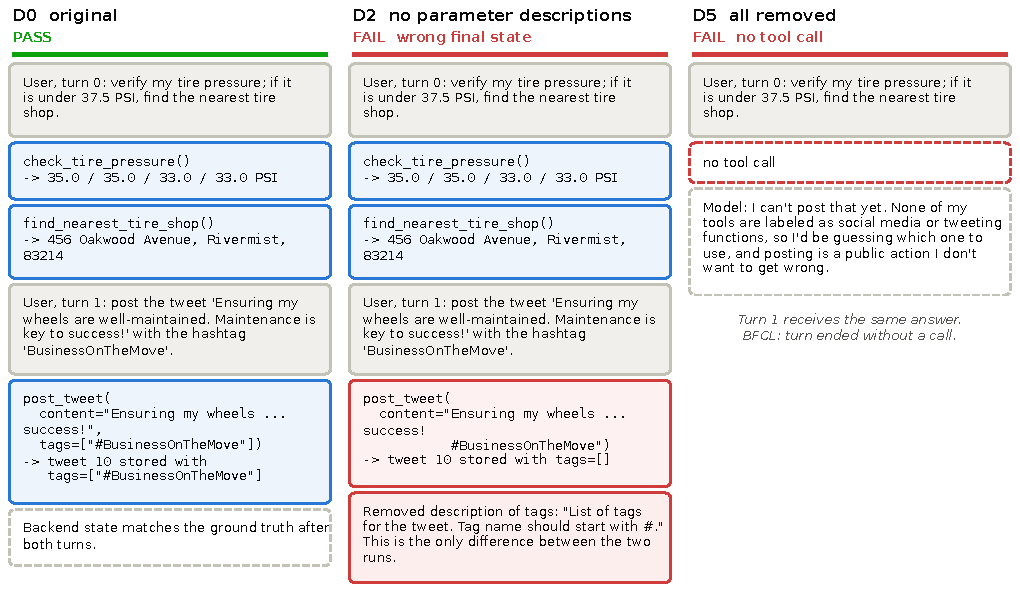
\includegraphics[width=0.7\linewidth]{fig0_trajectory}
\caption{One task under three conditions (Claude Haiku~5.5, BFCL task 78). With the original schema (D0) the hashtag goes in the \code{tags} list. Without parameter descriptions (D2) the first turn is identical, but the hashtag is folded into the tweet body and the final state no longer matches. With names and descriptions removed (D5) the model declines to guess which tool posts.}
\label{fig:trajectory}
\end{figure}

Cases were selected by one rule per model in its default reasoning setting: among tasks that pass in D0 and fail in D2, take the one with the fewest ground-truth calls (lowest id on ties), and show it in D0, D2 and D5. The rule favours short tasks so that the whole trajectory can be shown.

\paragraph{Claude Haiku~5.5, task 78 (Figure~\ref{fig:trajectory}).} Turn~0 is identical in D0 and D2. In turn~1, D0 passes the hashtag as \code{tags=["\#BusinessOnTheMove"]}; D2 folds it into \code{content}, so the backend records a tweet with no tags. The only information that changed is the removed \code{tags} description. In D5 the model never calls a tool and says it will not guess which unlabeled tool posts to social media.

\paragraph{Gemma~4 26B-A4B, task 11.} The user asks to list the files in a \code{/temp} directory (which does not exist) and tweet their names with \code{\#fileshowcase}. D0 and D2 both wander in turn~0 and end it in the correct state; turn~1 is decided by the same hashtag-in-content error. In D5 the single call is \code{get\_user\_stats(username="ls -a /temp")}: a Twitter tool with the shell command as its argument.

\paragraph{GPT-6 Luna, task 177.} The user books a flight from Los Angeles to Tokyo and asks to confirm the booking's details. D2 shows a recovered construction failure and an unrecovered selection failure: it first calls \code{get\_flight\_cost} with city names (the removed descriptions said airport codes), gets an error, corrects to \code{LAX} and \code{HND}, and books; in turn~1 D0 calls \code{retrieve\_invoice} while D2 calls \code{get\_booking\_history}, and BFCL requires the invoice output. In D5 the model answers with an essay about verifying itineraries and never calls a tool.

\paragraph{Qwen3-30B-A3B, task 42.} The user asks to create a file in an existing \code{Lectures} folder. In D0, after \code{cd Lectures} fails, the model calls \code{pwd}, finds it is already inside the folder, and proceeds. In D2 it stops after the failed \code{cd}, and in turn~1 creates a second \code{Lectures} folder inside the first, so the directory tree has an extra folder. Nothing about the documentation of the tools involved differs between D0 and D2; the run diverged on a near-tie decision and the evaluator is strict about state. In D5 the model tries eleven tools with guessed arguments and gives up.

Every decoded call and its result under D0, D2 and D5 follows. Results are truncated to about 100 characters; execution errors are in red.

\rawinput tables/cases.tex

\end{document}
